% =============================================================================
% BidForge — Freelance Marketplace Bidding Engine
% Professional Project Report
% =============================================================================
\documentclass[12pt, a4paper]{report}

% --- Packages ----------------------------------------------------------------
\usepackage[utf8]{inputenc}
\usepackage[T1]{fontenc}
\usepackage{lmodern}
\usepackage[margin=1in]{geometry}
\usepackage{graphicx}
\usepackage{xcolor}
\usepackage{titlesec}
\usepackage{titling}
\usepackage{fancyhdr}
\usepackage{hyperref}
\usepackage{listings}
\usepackage{booktabs}
\usepackage{longtable}
\usepackage{tabularx}
\usepackage{multirow}
\usepackage{enumitem}
\usepackage{amsmath}
\usepackage{amssymb}
\usepackage{float}
\usepackage{caption}
\usepackage{subcaption}
\usepackage{tikz}
\usepackage{pgfplots}
\usepackage{tcolorbox}
\usepackage{mdframed}
\usepackage{setspace}
\usepackage{parskip}
\usepackage{tocloft}
\usepackage{pdfpages}
\usepackage{background}

\pgfplotsset{compat=1.18}
\usetikzlibrary{shapes.geometric, arrows.meta, positioning, fit, calc}

% --- Page Border (black border on every page) --------------------------------
\backgroundsetup{
  scale=1,
  color=black,
  opacity=1,
  angle=0,
  position=current page.center,
  contents={%
    
\begin{tikzpicture}[remember picture, overlay]
      \draw[black, line width=1.5pt]
        ([shift={(0.5cm,-0.5cm)}]current page.north west) rectangle
        ([shift={(-0.5cm,0.5cm)}]current page.south east);
    \end{tikzpicture}%
  }
}

% --- Colors ------------------------------------------------------------------
\definecolor{forestblack}{HTML}{06120E}
\definecolor{emerald}{HTML}{10B981}
\definecolor{emeralddark}{HTML}{047857}
\definecolor{gold}{HTML}{FBBF24}
\definecolor{codebg}{HTML}{1A1A2E}
\definecolor{codetext}{HTML}{E0E0E0}
\definecolor{codekey}{HTML}{10B981}
\definecolor{codecomment}{HTML}{6B7280}
\definecolor{codestring}{HTML}{FBBF24}
\definecolor{sectioncolor}{HTML}{047857}

% --- Hyperref Setup ----------------------------------------------------------
\hypersetup{
  colorlinks=true,
  linkcolor=emeralddark,
  urlcolor=emerald,
  citecolor=emeralddark,
  pdftitle={BidForge -- Freelance Marketplace Bidding Engine},
  pdfauthor={Dhyey Joshi},
  pdfsubject={Project Report},
}

% --- Code Listings Setup -----------------------------------------------------
\lstdefinestyle{pythonstyle}{
  backgroundcolor=\color{codebg},
  basicstyle=\ttfamily\small\color{codetext},
  keywordstyle=\color{codekey}\bfseries,
  commentstyle=\color{codecomment}\itshape,
  stringstyle=\color{codestring},
  numberstyle=\tiny\color{codecomment},
  numbers=left,
  numbersep=8pt,
  breaklines=true,
  frame=single,
  rulecolor=\color{gray!40},
  tabsize=4,
  showstringspaces=false,
  captionpos=b,
  xleftmargin=1em,
  framexleftmargin=1em,
}

\lstdefinestyle{sqlstyle}{
  backgroundcolor=\color{codebg},
  basicstyle=\ttfamily\small\color{codetext},
  keywordstyle=\color{codekey}\bfseries,
  commentstyle=\color{codecomment}\itshape,
  stringstyle=\color{codestring},
  numbers=left,
  numbersep=8pt,
  breaklines=true,
  frame=single,
  rulecolor=\color{gray!40},
  tabsize=4,
  showstringspaces=false,
  morekeywords={CREATE, TABLE, PRIMARY, KEY, FOREIGN, REFERENCES, INTEGER, TEXT, FLOAT, DATETIME, UNIQUE, NOT, NULL, DEFAULT, JSON, CASCADE, ON, DELETE, INDEX},
  xleftmargin=1em,
  framexleftmargin=1em,
}

\lstdefinestyle{bashstyle}{
  backgroundcolor=\color{codebg},
  basicstyle=\ttfamily\small\color{codetext},
  keywordstyle=\color{codekey},
  commentstyle=\color{codecomment}\itshape,
  frame=single,
  rulecolor=\color{gray!40},
  breaklines=true,
  showstringspaces=false,
  xleftmargin=1em,
  framexleftmargin=1em,
}

\lstset{style=pythonstyle, language=Python}

% --- Section Formatting ------------------------------------------------------
\titleformat{\chapter}[display]
  {\normalfont\Huge\bfseries\color{sectioncolor}}
  {\chaptertitlename\ \thechapter}{20pt}{\Huge}
\titleformat{\section}
  {\normalfont\Large\bfseries\color{sectioncolor}}
  {\thesection}{1em}{}
\titleformat{\subsection}
  {\normalfont\large\bfseries\color{emeralddark}}
  {\thesubsection}{1em}{}

% --- Header/Footer -----------------------------------------------------------
\pagestyle{fancy}
\fancyhf{}
\fancyhead[L]{\small\textit{BidForge --- Freelance Marketplace Bidding Engine}}
\fancyhead[R]{\small\textit{\leftmark}}
\fancyfoot[C]{\thepage}
\renewcommand{\headrulewidth}{0.4pt}
\renewcommand{\footrulewidth}{0.4pt}

% --- Custom Environments -----------------------------------------------------
\newtcolorbox{infobox}[1][]{
  colback=emerald!5,
  colframe=emerald!60!black,
  fonttitle=\bfseries,
  title=#1,
  arc=2mm,
}

\newtcolorbox{warnbox}[1][]{
  colback=gold!10,
  colframe=gold!80!black,
  fonttitle=\bfseries,
  title=#1,
  arc=2mm,
}

% =============================================================================
\begin{document}

% --- Title Page --------------------------------------------------------------
\begin{titlepage}
  \centering
  \vspace*{2cm}

  {\Huge\bfseries\color{sectioncolor} BidForge}\\[0.5cm]
  {\LARGE Freelance Marketplace Bidding Engine}\\[1.5cm]

  \rule{\textwidth}{1pt}\\[0.5cm]
  {\Large\textit{Bids ranked on fit, not just price.}}\\[0.3cm]
  {\large A full-stack platform where a scoring engine weighs\\skill match, price fit, and past ratings.}\\[0.5cm]
  \rule{\textwidth}{1pt}\\[2cm]

  {\Large\textbf{Project Report}}\\[1.5cm]

  \begin{tabular}{rl}
    \textbf{Author:}      & Dhyey Joshi \\[0.3cm]
    \textbf{Repository:}   & \href{https://github.com/dhyeyjoshi07/Freelance-Marketplace-Bidding-Engine}{\texttt{github.com/dhyeyjoshi07/Freelance-Marketplace-Bidding-Engine}} \\[0.3cm]
    \textbf{Tech Stack:}   & Python 3.14, FastAPI, SQLAlchemy, SQLite \\[0.3cm]
    \textbf{Tests:}        & 91 (40 unit + 28 scoring + 23 integration) \\[0.3cm]
    \textbf{License:}      & MIT \\[0.3cm]
    \textbf{Date:}         & October 2026 \\
  \end{tabular}

  \vfill
  {\small Built with FastAPI \(\cdot\) SQLAlchemy \(\cdot\) Vanilla HTML/CSS/JS}
\end{titlepage}

% --- Table of Contents -------------------------------------------------------
\tableofcontents
\newpage

% =============================================================================
\chapter{Abstract}
% =============================================================================

BidForge is a full-stack freelance marketplace platform that replaces the traditional ``lowest bid wins'' model with a \textbf{fit-based ranking engine}. When a freelancer submits a bid on a project, the system automatically computes a composite \texttt{match\_score} by evaluating three dimensions: skill overlap between the freelancer and the project's requirements (weighted at 45\%), how well the bid amount fits the client's budget range (30\%), and the freelancer's historical rating (25\%). Bids are then presented to clients in ranked order, so the most qualified candidates surface first regardless of price.

The system is built on \textbf{FastAPI} with \textbf{SQLAlchemy} ORM over SQLite, implementing a rigorous object-oriented architecture: an abstract base class hierarchy for users, a polymorphic match engine with overridable scoring components, operator-overloaded dataclasses for heap-based bid ranking, encapsulated state machines for project lifecycle management, and four custom exception types for domain-specific error handling. The frontend is a dark-themed glassmorphism interface built with vanilla HTML, CSS, and JavaScript.

The project is validated by \textbf{91 automated tests} spanning unit tests for OOP models, algorithmic tests for the scoring engine, and full API lifecycle integration tests. All tests pass with zero application warnings.

% =============================================================================
\chapter{Introduction}
% =============================================================================

\section{Problem Statement}

Traditional freelance marketplaces like Upwork and Fiverr rank bids primarily by price, creating a race to the bottom that penalizes experienced freelancers and leaves clients sifting through low-quality proposals. The core problem is \textbf{one-dimensional ranking}: when the only visible metric is price, both parties lose.

\section{Proposed Solution}

BidForge introduces a \textbf{multi-dimensional scoring engine} that evaluates each bid across three orthogonal dimensions:

\begin{enumerate}[label=\arabic*.]
  \item \textbf{Skill overlap} --- How many of the project's required skills does the freelancer possess?
  \item \textbf{Price fit} --- Does the bid amount fall within the client's budget range?
  \item \textbf{Past performance} --- What is the freelancer's average rating from prior projects?
\end{enumerate}

This produces a single composite score in $[0, 1]$ that captures ``overall fit,'' allowing clients to see the best candidates first without manually cross-referencing skills, prices, and reviews.

\section{Objectives}

\begin{itemize}[leftmargin=2em]
  \item Design and implement a full-stack web application with role-based authentication (client vs.\ freelancer).
  \item Build a configurable, polymorphic scoring engine with documented algorithmic complexity.
  \item Enforce project lifecycle integrity via encapsulated state machines and custom exceptions.
  \item Demonstrate advanced OOP patterns: ABC hierarchies, operator overloading, heap-based containers, and polymorphic method dispatch.
  \item Achieve comprehensive test coverage across all layers (models, services, API).
\end{itemize}

\section{Scope}

The project encompasses five milestones:
\begin{enumerate}[label=\textbf{M\arabic*:}]
  \item Core models and database schema
  \item OOP engine (match scoring + ranked bid queue)
  \item REST API layer with JWT authentication
  \item Frontend dashboards (landing page, client dashboard, freelancer dashboard)
  \item Integration, seed data, and documentation
\end{enumerate}

% =============================================================================
\chapter{System Design}
% =============================================================================

\section{Architecture Overview}

BidForge follows a \textbf{three-tier architecture}:

\begin{center}
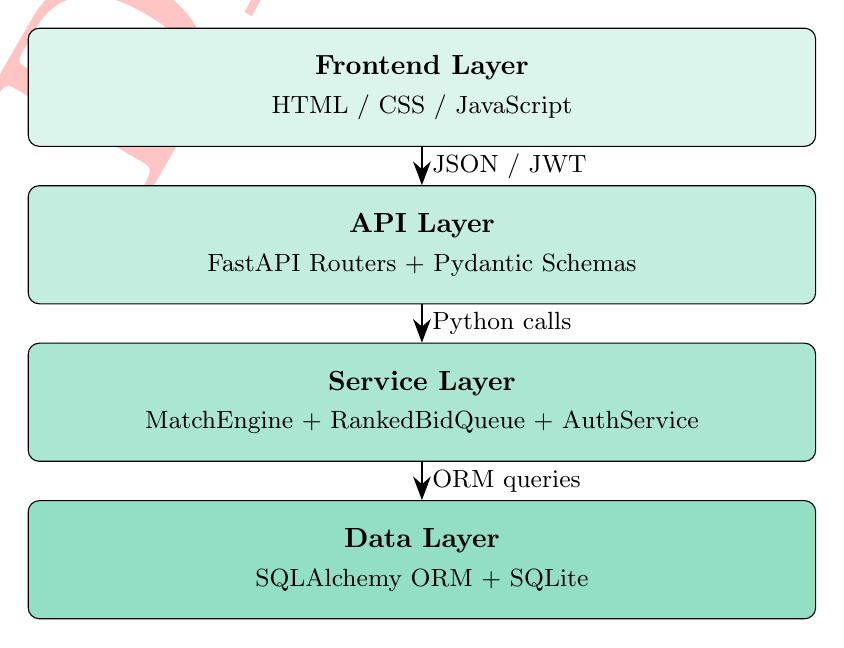
\begin{tikzpicture}[
  tier/.style={draw, rounded corners, minimum width=10cm, minimum height=1.5cm, align=center, font=\bfseries},
  arrow/.style={-{Stealth[length=3mm]}, thick},
]
  \node[tier, fill=emerald!15] (frontend) at (0,4) {Frontend Layer\\[2pt]\normalfont\small HTML / CSS / JavaScript};
  \node[tier, fill=emerald!25] (api) at (0,2) {API Layer\\[2pt]\normalfont\small FastAPI Routers + Pydantic Schemas};
  \node[tier, fill=emerald!35] (service) at (0,0) {Service Layer\\[2pt]\normalfont\small MatchEngine + RankedBidQueue + AuthService};
  \node[tier, fill=emerald!45] (data) at (0,-2) {Data Layer\\[2pt]\normalfont\small SQLAlchemy ORM + SQLite};

  \draw[arrow] (frontend) -- (api) node[midway, right, font=\small] {JSON / JWT};
  \draw[arrow] (api) -- (service) node[midway, right, font=\small] {Python calls};
  \draw[arrow] (service) -- (data) node[midway, right, font=\small] {ORM queries};
\end{tikzpicture}
\end{center}

\section{Class Hierarchy}

The core OOP design uses an abstract base class hierarchy for users and a polymorphic strategy pattern for the match engine:

\begin{center}
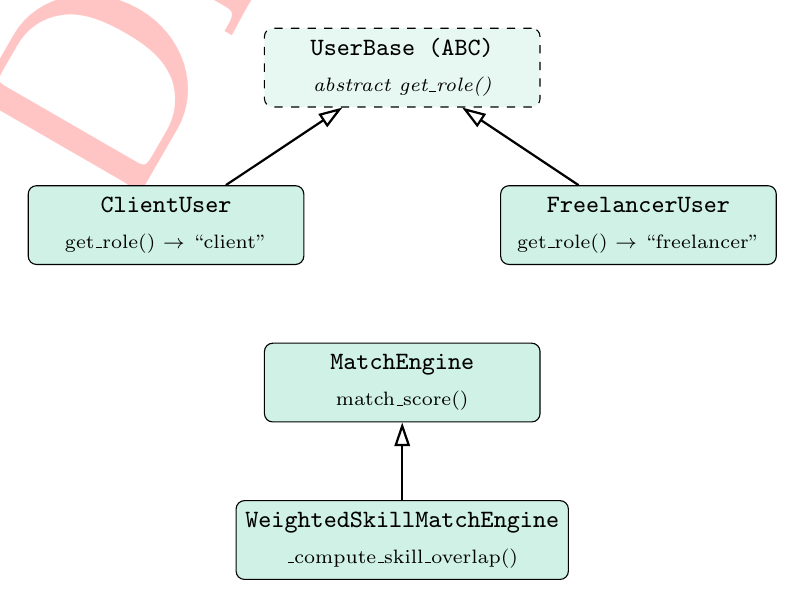
\begin{tikzpicture}[
  class/.style={draw, rectangle, rounded corners=3pt, minimum width=3.5cm, minimum height=1cm, align=center, font=\ttfamily\small},
  abstract/.style={class, fill=emerald!10, dashed},
  concrete/.style={class, fill=emerald!20},
  arrow/.style={-{Triangle[open, length=3mm]}, thick},
]
  % User hierarchy
  \node[abstract] (userbase) at (0,3) {UserBase (ABC)\\[2pt]\normalfont\itshape\scriptsize abstract get\_role()};
  \node[concrete] (client) at (-3,1) {ClientUser\\[2pt]\normalfont\scriptsize get\_role() $\to$ ``client''};
  \node[concrete] (freelancer) at (3,1) {FreelancerUser\\[2pt]\normalfont\scriptsize get\_role() $\to$ ``freelancer''};

  \draw[arrow] (client) -- (userbase);
  \draw[arrow] (freelancer) -- (userbase);

  % MatchEngine hierarchy
  \node[concrete] (engine) at (0,-1) {MatchEngine\\[2pt]\normalfont\scriptsize match\_score()};
  \node[concrete] (weighted) at (0,-3) {WeightedSkillMatchEngine\\[2pt]\normalfont\scriptsize \_compute\_skill\_overlap()};

  \draw[arrow] (weighted) -- (engine);
\end{tikzpicture}
\end{center}

\section{Database Schema}

The application uses five tables in SQLite via SQLAlchemy:

\begin{center}
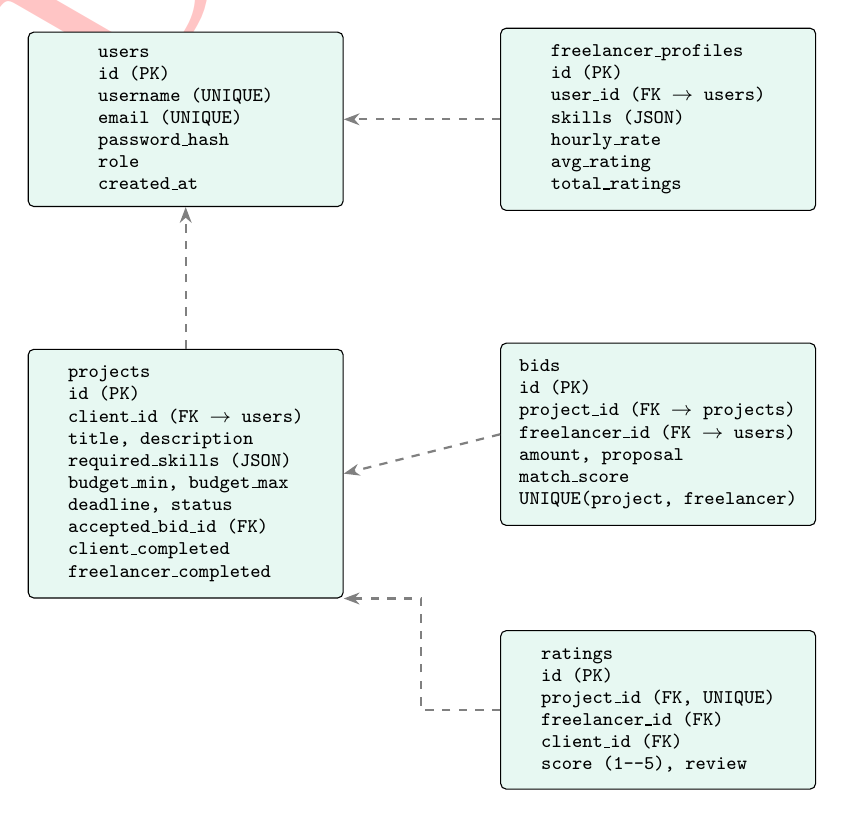
\begin{tikzpicture}[
  table/.style={draw, rectangle, rounded corners=2pt, minimum width=4cm, align=left, font=\ttfamily\scriptsize, inner sep=6pt},
  fk/.style={-{Stealth[length=2mm]}, thick, dashed, gray},
]
  \node[table, fill=emerald!10] (users) at (0,0) {
    \textbf{users}\\
    id (PK)\\
    username (UNIQUE)\\
    email (UNIQUE)\\
    password\_hash\\
    role\\
    created\_at
  };

  \node[table, fill=emerald!10] (profiles) at (6,0) {
    \textbf{freelancer\_profiles}\\
    id (PK)\\
    user\_id (FK $\to$ users)\\
    skills (JSON)\\
    hourly\_rate\\
    avg\_rating\\
    total\_ratings
  };

  \node[table, fill=emerald!10] (projects) at (0,-4.5) {
    \textbf{projects}\\
    id (PK)\\
    client\_id (FK $\to$ users)\\
    title, description\\
    required\_skills (JSON)\\
    budget\_min, budget\_max\\
    deadline, status\\
    accepted\_bid\_id (FK)\\
    client\_completed\\
    freelancer\_completed
  };

  \node[table, fill=emerald!10] (bids) at (6,-4) {
    \textbf{bids}\\
    id (PK)\\
    project\_id (FK $\to$ projects)\\
    freelancer\_id (FK $\to$ users)\\
    amount, proposal\\
    match\_score\\
    UNIQUE(project, freelancer)
  };

  \node[table, fill=emerald!10] (ratings) at (6,-7.5) {
    \textbf{ratings}\\
    id (PK)\\
    project\_id (FK, UNIQUE)\\
    freelancer\_id (FK)\\
    client\_id (FK)\\
    score (1--5), review
  };

  \draw[fk] (profiles.west) -- (users.east);
  \draw[fk] (projects.north) -- (users.south);
  \draw[fk] (bids.west) -- (projects.east);
  \draw[fk] (ratings.west) -- ++(-1,0) |- (projects.south east);
\end{tikzpicture}
\end{center}

\textbf{Key design decisions:}
\begin{itemize}
  \item \textbf{Skills as JSON arrays} --- enables flexible set-based matching via Python \texttt{set} intersection without join tables.
  \item \textbf{Denormalized \texttt{avg\_rating}} --- incrementally updated on each new rating, avoiding expensive aggregation queries.
  \item \textbf{Dual-completion flags} --- \texttt{client\_completed} and \texttt{freelancer\_completed} integers (0/1) enforce mutual confirmation.
\end{itemize}

% =============================================================================
\chapter{Implementation}
% =============================================================================

\section{Scoring Algorithm}

The match engine computes a weighted composite score for each bid:

\begin{equation}
  \texttt{match\_score} = w_s \cdot S_{\text{skill}} + w_p \cdot S_{\text{price}} + w_r \cdot S_{\text{rating}}
\end{equation}

where $w_s = 0.45$, $w_p = 0.30$, $w_r = 0.25$ (configurable in \texttt{config.py}).

\subsection{Skill Overlap ($S_{\text{skill}}$)}

Uses Python \texttt{set} intersection for $O(\min(m, n))$ matching:

\begin{equation}
  S_{\text{skill}} = \frac{|\text{required} \cap \text{offered}|}{|\text{required}|}
\end{equation}

If $|\text{required}| = 0$, the score is 1.0 (any freelancer is a full match).

\begin{lstlisting}[caption={Skill overlap computation}, language=Python]
def _compute_skill_overlap(self, freelancer_skills, required_skills):
    if not required_skills:
        return 1.0
    required = set(s.lower().strip() for s in required_skills)
    offered = set(s.lower().strip() for s in freelancer_skills)
    overlap = required & offered
    return len(overlap) / len(required)
\end{lstlisting}

\subsection{Price Fit ($S_{\text{price}}$)}

Scores how well the bid amount fits the client's budget range:

\[
S_{\text{price}} =
\begin{cases}
  1.0 & \text{if } b_{\min} \leq \text{bid} \leq b_{\max} \\[4pt]
  \dfrac{\text{bid}}{b_{\min}} & \text{if bid} < b_{\min} \\[6pt]
  \max\!\left(0,\; 1 - \dfrac{\text{bid} - b_{\max}}{b_{\max}}\right) & \text{if bid} > b_{\max}
\end{cases}
\]

Bids within the budget get a perfect 1.0. Bids outside the range decay linearly toward 0.0, reaching zero at \$0 (below) or $2 \times b_{\max}$ (above).

\subsection{Rating Normalization ($S_{\text{rating}}$)}

\[
S_{\text{rating}} =
\begin{cases}
  0.1 & \text{if avg\_rating} = 0 \text{ (new freelancer baseline)} \\
  \min\!\left(\dfrac{\text{avg\_rating}}{5.0},\; 1.0\right) & \text{otherwise}
\end{cases}
\]

New freelancers receive a 0.1 baseline so they are not completely penalized against rated freelancers.

\subsection{Polymorphic Extension}

The \texttt{WeightedSkillMatchEngine} subclass overrides \texttt{\_compute\_skill\_overlap()} to give 1.5$\times$ weight to designated ``bonus'' skills:

\begin{lstlisting}[caption={Polymorphic skill scoring override}, language=Python]
class WeightedSkillMatchEngine(MatchEngine):
    def __init__(self, bonus_skills=None, **kwargs):
        super().__init__(**kwargs)
        self.bonus_skills = {s.lower() for s in (bonus_skills or set())}

    def _compute_skill_overlap(self, freelancer_skills, required_skills):
        if not required_skills:
            return 1.0
        required = set(s.lower().strip() for s in required_skills)
        offered = set(s.lower().strip() for s in freelancer_skills)
        overlap = required & offered
        if not overlap:
            return 0.0
        weighted_score = sum(
            1.5 if skill in self.bonus_skills else 1.0
            for skill in overlap
        )
        max_score = sum(
            1.5 if skill in self.bonus_skills else 1.0
            for skill in required
        )
        return weighted_score / max_score
\end{lstlisting}

\section{Operator Overloading \& Heap-Based Ranking}

The \texttt{BidRanked} dataclass implements \textbf{inverted comparison operators} so Python's \texttt{heapq} (a min-heap) functions as a max-heap:

\begin{lstlisting}[caption={Inverted comparison for max-heap behavior}, language=Python]
@dataclass(order=False)
class BidRanked:
    bid_id: int
    match_score: float
    # ... additional fields ...

    def __lt__(self, other):
        """Higher match_score sorts first (inverted for min-heap)."""
        return self.match_score > other.match_score

    def __gt__(self, other):
        return self.match_score < other.match_score
\end{lstlisting}

This inversion means:
\begin{itemize}
  \item \texttt{sorted(bids)} returns highest-score-first order.
  \item \texttt{heapq.heappop()} returns the highest-scoring bid.
\end{itemize}

\subsection{RankedBidQueue}

The \texttt{RankedBidQueue} wraps Python's \texttt{heapq} module with a secondary index for $O(1)$ lookup:

\begin{table}[H]
\centering
\caption{RankedBidQueue time complexity}
\begin{tabular}{@{}lcc@{}}
\toprule
\textbf{Operation} & \textbf{Complexity} & \textbf{Mechanism} \\
\midrule
Push & $O(\log n)$ & \texttt{heapq.heappush} \\
Peek / Pop & $O(\log n)$ & Skips stale entries via lazy deletion \\
Full ranking & $O(n \log n)$ & \texttt{sorted()} on active entries \\
Remove & $O(1)$ & Lazy deletion via \texttt{\_index} dict \\
Batch construction & $O(n)$ & \texttt{heapq.heapify} in \texttt{from\_bids()} \\
\bottomrule
\end{tabular}
\end{table}

\section{Project Status Machine}

Project lifecycle transitions are \textbf{encapsulated} --- status is never mutated directly:

\begin{center}
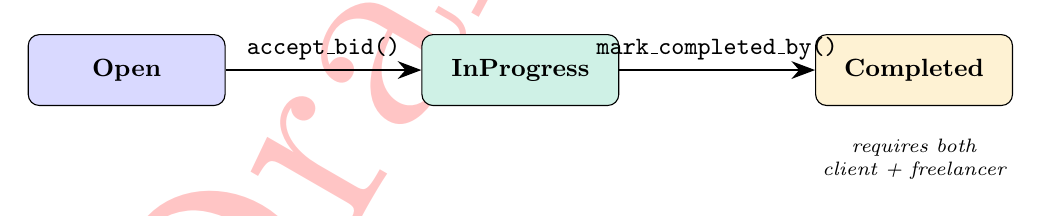
\begin{tikzpicture}[
  state/.style={draw, rounded corners, minimum width=2.5cm, minimum height=0.9cm, align=center, font=\bfseries\small},
  arrow/.style={-{Stealth[length=3mm]}, thick},
]
  \node[state, fill=blue!15] (open) at (0,0) {Open};
  \node[state, fill=emerald!20] (ip) at (5,0) {InProgress};
  \node[state, fill=gold!20] (done) at (10,0) {Completed};

  \draw[arrow] (open) -- (ip) node[midway, above, font=\small\ttfamily] {accept\_bid()};
  \draw[arrow] (ip) -- (done) node[midway, above, font=\small\ttfamily] {mark\_completed\_by()};

  \node[below=0.3cm, font=\scriptsize\itshape, text width=2.5cm, align=center] at (done.south) {requires both\\client + freelancer};
\end{tikzpicture}
\end{center}

Invalid transitions (e.g., \texttt{Open} $\to$ \texttt{Completed}) raise \texttt{InvalidStatusTransitionError}.

\section{Custom Exception Handling}

Four domain-specific exceptions enforce business rules:

\begin{table}[H]
\centering
\caption{Custom exceptions and their HTTP mappings}
\begin{tabular}{@{}llc@{}}
\toprule
\textbf{Exception} & \textbf{Trigger} & \textbf{HTTP} \\
\midrule
\texttt{BidOnExpiredProjectError} & Bidding on closed/expired project & 400 \\
\texttt{DuplicateBidError} & Same freelancer bids twice & 409 \\
\texttt{InvalidBudgetError} & \texttt{budget\_min} $\geq$ \texttt{budget\_max} or negative & 400 \\
\texttt{InvalidStatusTransitionError} & Illegal state change & 400 \\
\bottomrule
\end{tabular}
\end{table}

Each exception is raised in the model/service layer and caught in the router layer to produce the correct HTTP response with a descriptive error message.

\section{Authentication}

Authentication uses \textbf{bcrypt} for password hashing and \textbf{JWT} tokens for stateless session management:

\begin{enumerate}
  \item \textbf{Registration:} Password is hashed with \texttt{bcrypt.hashpw()} using a random salt. Freelancers automatically receive an empty \texttt{FreelancerProfile}.
  \item \textbf{Login:} Password is verified via \texttt{bcrypt.checkpw()}. On success, a JWT is issued containing \texttt{sub} (user ID) and \texttt{role}.
  \item \textbf{Authorization:} The \texttt{require\_role()} dependency factory produces FastAPI \texttt{Depends()} callables that enforce role-based access per endpoint.
\end{enumerate}

\section{API Design}

The REST API is organized into four routers:

\begin{table}[H]
\centering
\caption{API endpoint summary (15 endpoints)}
\begin{tabular}{@{}llp{7cm}@{}}
\toprule
\textbf{Method} & \textbf{Path} & \textbf{Description} \\
\midrule
\multicolumn{3}{l}{\textit{Auth}} \\
POST & \texttt{/api/auth/register} & Register a new user \\
POST & \texttt{/api/auth/login} & Authenticate, returns JWT \\
GET  & \texttt{/api/auth/me} & Current user profile \\
\midrule
\multicolumn{3}{l}{\textit{Projects}} \\
POST & \texttt{/api/projects} & Create project (client only) \\
GET  & \texttt{/api/projects} & List open projects \\
GET  & \texttt{/api/projects/my} & User's own projects \\
GET  & \texttt{/api/projects/\{id\}} & Project detail \\
POST & \texttt{/api/projects/\{id\}/accept-bid} & Accept bid $\to$ InProgress \\
POST & \texttt{/api/projects/\{id\}/complete} & Dual-confirm completion \\
POST & \texttt{/api/projects/\{id\}/rate} & Rate freelancer (1--5) \\
\midrule
\multicolumn{3}{l}{\textit{Bids}} \\
POST & \texttt{/api/projects/\{id\}/bids} & Submit bid (auto-scored) \\
GET  & \texttt{/api/projects/\{id\}/bids} & Ranked bid list \\
GET  & \texttt{/api/freelancers/me/bids} & Freelancer's bids \\
\midrule
\multicolumn{3}{l}{\textit{Freelancers}} \\
GET  & \texttt{/api/freelancers/me} & View profile \\
PUT  & \texttt{/api/freelancers/me} & Update skills/rate \\
\bottomrule
\end{tabular}
\end{table}

\section{Frontend}

The frontend consists of three pages built with vanilla HTML, CSS, and JavaScript:

\begin{enumerate}
  \item \textbf{Landing Page} (\texttt{index.html}) --- Login/register with role selection (Client or Freelancer). Dark-themed glassmorphism card with auto-login after registration.
  \item \textbf{Client Dashboard} (\texttt{client.html}) --- Post new projects, view own projects with status badges, see ranked bids with animated score-breakdown bars, accept bids, mark projects complete, and rate freelancers with interactive star ratings.
  \item \textbf{Freelancer Dashboard} (\texttt{freelancer.html}) --- Browse open projects with skill-match highlighting, submit bids with real-time score feedback, track bid status, manage profile (skills and hourly rate).
\end{enumerate}

\textbf{Design system:}
\begin{itemize}
  \item \textbf{Palette:} Deep forest black (\texttt{\#06120e}) base, emerald gradients (\texttt{\#10b981} $\to$ \texttt{\#047857}), gold accent (\texttt{\#fbbf24}).
  \item \textbf{Typography:} Inter (body) and Outfit (headings) from Google Fonts.
  \item \textbf{Components:} Glassmorphism cards, animated score-breakdown bars (emerald = skill, gold = rating, teal = price), status badges, skill chips with match highlighting, toast notifications.
\end{itemize}

% =============================================================================
\chapter{OOP Concepts Matrix}
% =============================================================================

This chapter maps each required OOP concept to its concrete implementation:

\begin{table}[H]
\centering
\caption{OOP concepts and their implementations in BidForge}
\begin{tabular}{@{}p{3.5cm}p{3cm}p{7cm}@{}}
\toprule
\textbf{Concept} & \textbf{Location} & \textbf{Implementation} \\
\midrule
Abstraction & \texttt{UserBase} (ABC) & Abstract method \texttt{get\_role()} forces subclasses to declare their role. Cannot be instantiated directly. \\[4pt]

Inheritance & \texttt{ClientUser}, \texttt{FreelancerUser} & Both inherit from \texttt{UserBase} and implement \texttt{get\_role()} returning \texttt{"client"} or \texttt{"freelancer"}. \\[4pt]

Polymorphism & \texttt{MatchEngine} & Base class defines \texttt{\_compute\_skill\_overlap()}, \texttt{\_compute\_price\_fit()}, \texttt{\_normalize\_rating()} as overridable methods. \texttt{WeightedSkillMatchEngine} overrides skill overlap with weighted scoring. \\[4pt]

Operator overloading & \texttt{BidRanked} & Implements \texttt{\_\_lt\_\_}, \texttt{\_\_gt\_\_}, \texttt{\_\_eq\_\_}, \texttt{\_\_le\_\_}, \texttt{\_\_ge\_\_}, \texttt{\_\_hash\_\_} with inverted comparison for max-heap behavior. \\[4pt]

Encapsulation & \texttt{Project} & Status transitions only via \texttt{accept\_bid()} and \texttt{mark\_completed\_by()} methods. Direct mutation is never used. \\[4pt]

Exception handling & \texttt{exceptions.py} & 5 custom exception classes with contextual error messages, caught in routers and mapped to HTTP status codes. \\[4pt]

Containers & \texttt{RankedBidQueue} & Wraps \texttt{heapq} with lazy deletion and $O(1)$ index dict. Factory \texttt{from\_bids()} uses $O(n)$ heapify. \\[4pt]

Dataclass & \texttt{BidRanked} & \texttt{@dataclass(order=False)} with custom comparators, used as heap elements. \\
\bottomrule
\end{tabular}
\end{table}

% =============================================================================
\chapter{Testing}
% =============================================================================

\section{Test Suite Overview}

The project includes \textbf{91 automated tests} organized into three test modules:

\begin{table}[H]
\centering
\caption{Test distribution by module}
\begin{tabular}{@{}lcp{7cm}@{}}
\toprule
\textbf{Module} & \textbf{Tests} & \textbf{Coverage} \\
\midrule
\texttt{test\_models.py} & 40 & ABC hierarchy, operator overloading (6 tests), project transitions (7 tests), budget validation (5 tests), freelancer rating (4 tests), custom exceptions (5 tests), RankedBidQueue (9 tests) \\[4pt]
\texttt{test\_match\_engine.py} & 28 & Skill overlap (6 tests), price fit (9 tests), rating normalization (4 tests), composite score (5 tests), WeightedSkillMatchEngine (4 tests) \\[4pt]
\texttt{test\_api.py} & 23 & Auth flow (6 tests), freelancer profile (3 tests), projects CRUD (6 tests), bids (5 tests), full lifecycle (1 test), ratings (2 tests) \\
\bottomrule
\end{tabular}
\end{table}

\section{Test Results}

\begin{lstlisting}[style=bashstyle, caption={Final test run output}]
$ python3 -m pytest tests/ -v
======================== 91 passed, 1 warning in 9.79s ========================
\end{lstlisting}

The single remaining warning is a third-party Starlette/httpx deprecation notice, not from application code.

\section{Key Test Scenarios}

\begin{enumerate}
  \item \textbf{ABC enforcement:} Verifies that \texttt{UserBase} cannot be instantiated directly (\texttt{TypeError}).
  \item \textbf{Operator inversion:} Confirms \texttt{BidRanked(score=0.9) < BidRanked(score=0.5)} due to inverted \texttt{\_\_lt\_\_}.
  \item \textbf{Heapq integration:} Verifies that \texttt{heapq.heappop()} returns the highest-scoring bid first.
  \item \textbf{Dual completion:} Tests that a project transitions to \texttt{Completed} only after both client and freelancer confirm.
  \item \textbf{Full lifecycle:} End-to-end test covering registration $\to$ project creation $\to$ bid submission $\to$ bid acceptance $\to$ dual completion $\to$ rating.
\end{enumerate}

% =============================================================================
\chapter{Seed Data \& Demonstration}
% =============================================================================

The \texttt{seed.py} script populates the database with realistic demo data:

\begin{table}[H]
\centering
\caption{Seed data summary}
\begin{tabular}{@{}lr@{}}
\toprule
\textbf{Entity} & \textbf{Count} \\
\midrule
Clients & 3 \\
Freelancers (with varied skills and ratings) & 5 \\
Projects (across different domains) & 6 \\
Bids (with computed match scores) & 13 \\
\bottomrule
\end{tabular}
\end{table}

\subsection{Example: Ranked Bids for ``FastAPI Microservice Platform''}

\begin{table}[H]
\centering
\caption{Ranked bid output for Project \#1 (budget: \$3,000--\$12,000)}
\begin{tabular}{@{}clllr@{}}
\toprule
\textbf{Rank} & \textbf{Freelancer} & \textbf{Skills} & \textbf{Bid} & \textbf{Score} \\
\midrule
\#1 & dev\_alice & python, fastapi, sql, docker, aws & \$8,000 & 0.975 \\
\#2 & dev\_charlie & python, react, sql, redis, graphql & \$9,500 & 0.758 \\
\#3 & dev\_diana & python, pytorch, tensorflow, sql, docker & \$11,000 & 0.662 \\
\bottomrule
\end{tabular}
\end{table}

\textbf{Analysis:} dev\_alice ranks first despite not being the cheapest bid because she matches 4/4 required skills (vs.\ 2/4 for the others) and has a 4.5-star rating. The scoring engine correctly surfaces the best-fit candidate.

% =============================================================================
\chapter{Project Structure}
% =============================================================================

\begin{lstlisting}[style=bashstyle, caption={Complete project file tree (41 files)}]
freelance-marketplace/
+-- backend/                     # FastAPI + SQLAlchemy
|   +-- app.py                   # App factory, lifespan, static mount
|   +-- config.py                # DB URL, JWT secret, match weights
|   +-- database.py              # Engine, session, Base
|   +-- dependencies.py          # get_db, get_current_user, require_role()
|   +-- exceptions.py            # 5 custom exception classes
|   +-- models/
|   |   +-- enums.py             # ProjectStatus, UserRole
|   |   +-- user.py              # User ABC + FreelancerProfile
|   |   +-- project.py           # Project with status machine
|   |   +-- bid.py               # Bid ORM + BidRanked dataclass + Rating
|   +-- schemas/                 # Pydantic request/response models
|   +-- routers/
|   |   +-- auth.py              # Register, login, me
|   |   +-- projects.py          # CRUD + accept + complete
|   |   +-- bids.py              # Submit + ranked list
|   |   +-- freelancers.py       # Profile + ratings
|   +-- services/
|       +-- auth_service.py      # bcrypt + JWT
|       +-- match_engine.py      # MatchEngine + WeightedSkillMatchEngine
|       +-- ranking.py           # RankedBidQueue (heapq-based)
+-- frontend/                    # Vanilla HTML/CSS/JS
|   +-- index.html, client.html, freelancer.html
|   +-- css/styles.css           # Design system (740+ lines)
|   +-- js/api.js, auth.js, client.js, freelancer.js
+-- tests/
|   +-- test_models.py           # 40 unit tests
|   +-- test_match_engine.py     # 28 scoring tests
|   +-- test_api.py              # 23 integration tests
+-- seed.py, run.py, requirements.txt, LICENSE, README.md
\end{lstlisting}

% =============================================================================
\chapter{Conclusion}
% =============================================================================

\section{Achievements}

BidForge demonstrates that a freelance marketplace can move beyond ``lowest bid wins'' by implementing a \textbf{multi-dimensional scoring engine} that evaluates skill overlap, price fit, and past performance. The project successfully implements:

\begin{itemize}
  \item A \textbf{three-component scoring formula} with configurable weights and polymorphic extension points.
  \item A \textbf{heap-based ranking system} with $O(\log n)$ insertion and $O(1)$ lazy deletion.
  \item A \textbf{rigorous OOP architecture} with ABC hierarchies, operator overloading, encapsulated state machines, and custom exceptions.
  \item A \textbf{full-stack web application} with role-based JWT authentication, a dark-themed glassmorphism frontend, and 15 REST API endpoints.
  \item \textbf{91 automated tests} covering unit, algorithmic, and integration layers.
\end{itemize}

\section{Limitations \& Future Work}

\begin{itemize}
  \item \textbf{Real-time updates:} The current architecture uses polling; WebSocket integration would enable live bid ranking updates.
  \item \textbf{NLP-based skill matching:} Replacing exact-match set intersection with semantic similarity (e.g., Word2Vec or sentence transformers) would improve matching quality.
  \item \textbf{PostgreSQL migration:} SQLite is sufficient for demonstration but lacks concurrent write support for production use.
  \item \textbf{Payment integration:} Adding Stripe or a similar payment gateway would complete the marketplace flow.
  \item \textbf{Deployment:} Containerization with Docker and deployment to a cloud provider (e.g., Railway, Render) would make the demo publicly accessible.
\end{itemize}

\section{Key Takeaways}

\begin{enumerate}
  \item \textbf{Scoring beats sorting:} A composite fitness score that weights multiple dimensions produces better candidate rankings than single-axis sorting.
  \item \textbf{OOP enforces invariants:} Encapsulated state machines and custom exceptions prevent invalid state transitions at the design level, not just via validation.
  \item \textbf{Operator overloading enables idiomatic containers:} Inverting \texttt{\_\_lt\_\_} on a dataclass lets Python's built-in \texttt{heapq} and \texttt{sorted()} work as a max-heap without external libraries.
  \item \textbf{Polymorphism enables extension:} The strategy pattern on the match engine means scoring behavior can be changed by subclassing, not by modifying core code.
\end{enumerate}

% =============================================================================
\chapter*{References}
\addcontentsline{toc}{chapter}{References}
% =============================================================================

\begin{enumerate}[label={[\arabic*]}]
  \item FastAPI Documentation. \url{https://fastapi.tiangolo.com/}
  \item SQLAlchemy 2.0 Documentation. \url{https://docs.sqlalchemy.org/en/20/}
  \item Python \texttt{abc} --- Abstract Base Classes. \url{https://docs.python.org/3/library/abc.html}
  \item Python \texttt{heapq} --- Heap Queue Algorithm. \url{https://docs.python.org/3/library/heapq.html}
  \item Python \texttt{dataclasses} --- Data Classes. \url{https://docs.python.org/3/library/dataclasses.html}
  \item Pydantic V2 Documentation. \url{https://docs.pydantic.dev/latest/}
  \item bcrypt --- Modern Password Hashing. \url{https://pypi.org/project/bcrypt/}
  \item python-jose --- JSON Web Tokens. \url{https://pypi.org/project/python-jose/}
  \item pytest Documentation. \url{https://docs.pytest.org/}
  \item BidForge Source Code. \url{https://github.com/dhyeyjoshi07/Freelance-Marketplace-Bidding-Engine}
\end{enumerate}

\end{document}
